%%%
% Plantilla de Trabajo
% Modificación de una plantilla de Latex de Frits Wenneker para adaptarla 
% al castellano y a las necesidades de escribir informática y matemáticas.
%
% Editada por: Mario Román
%
% License:
% CC BY-NC-SA 3.0 (http://creativecommons.org/licenses/by-nc-sa/3.0/)
%%%

%%%%%%%%%%%%%%%%%%%%%%%%%%%%%%%%%%%%%%%%
% Short Sectioned Assignment
% LaTeX Template
% Version 1.0 (5/5/12)
%
% This template has been downloaded from:
% http://www.LaTeXTemplates.com
%
% Original author:
% Frits Wenneker (http://www.howtotex.com)
%
% License:
% CC BY-NC-SA 3.0 (http://creativecommons.org/licenses/by-nc-sa/3.0/)
%
%%%%%%%%%%%%%%%%%%%%%%%%%%%%%%%%%%%%%%%%%

%----------------------------------------------------------------------------------------
%	PAQUETES Y CONFIGURACIÓN DEL DOCUMENTO
%----------------------------------------------------------------------------------------

%%% Configuración del papel.
% fourier: Usa la fuente Adobe Utopia. (Comentando la línea usa la fuente normal)
\documentclass[paper=a4, fontsize=10pt, spanish]{scrartcl} 

%%% Castellano.
% noquoting: Permite uso de comillas no españolas.
% lcroman: Permite la enumeración con numerales romanos en minúscula.
% fontenc: Usa la fuente completa para que pueda copiarse correctamente del pdf.
\usepackage[spanish,es-noquoting,es-lcroman]{babel}
\usepackage[utf8]{inputenc}
\usepackage[T1]{fontenc}
\selectlanguage{spanish}

% Centra y formatea los títulos de sección.
% Quita la indentación de párrafos.
\usepackage{sectsty} % Allows customizing section commands
%\allsectionsfont{\centering \normalfont\scshape} % Make all sections centered, the default font and small caps
\setlength\parindent{0pt} % Removes all indentation from paragraphs - comment this line for an assignment with lots of text

% Permite elegir cabeceras y pies de página.
\usepackage{fancyhdr} % Custom headers and footers
\pagestyle{fancyplain} % Makes all pages in the document conform to the custom headers and footers
\fancyhead{} % No page header - if you want one, create it in the same way as the footers below
\fancyfoot[L]{} % Empty left footer
\fancyfoot[C]{} % Empty center footer
\fancyfoot[R]{\textit{Mario Román}} % Page numbering for right footer
\renewcommand{\headrulewidth}{0pt} % Remove header underlines
\renewcommand{\footrulewidth}{0pt} % Remove footer underlines
\setlength{\headheight}{13.6pt} % Customize the height of the header





%%% Matemáticas.
% Paquetes de la AMS. Para entornos de ecuaciones.
\usepackage{amsmath,amsfonts,amsthm}

% Incluye números entre secciones y ecuaciones.
\numberwithin{equation}{section} % Number equations within sections (i.e. 1.1, 1.2, 2.1, 2.2 instead of 1, 2, 3, 4)
\numberwithin{figure}{section} % Number figures within sections (i.e. 1.1, 1.2, 2.1, 2.2 instead of 1, 2, 3, 4)
\numberwithin{table}{section} % Number tables within sections (i.e. 1.1, 1.2, 2.1, 2.2 instead of 1, 2, 3, 4)


\usepackage{graphicx}


%----------------------------------------------------------------------------------------
%	TÍTULO
%----------------------------------------------------------------------------------------
% Título con las líneas horizontales, nombres y fecha.

\newcommand{\horrule}[1]{\rule{\linewidth}{#1}} % Create horizontal rule command with 1 argument of height

\title{
  \normalfont \normalsize 
  \textsc{Universidad de Granada.} \\ [25pt] % Your university, school and/or department name(s)
  \horrule{0.5pt} \\[0.4cm] % Thin top horizontal rule
  \huge Título \\ % The assignment title
  \horrule{2pt} \\[0.5cm] % Thick bottom horizontal rule
}

\author{Autor} % Your name

\date{\normalsize\today} % Today's date or a custom date



%----------------------------------------------------------------------------------------
%	DOCUMENTO
%----------------------------------------------------------------------------------------


\begin{document}
%\maketitle % Escribe el título
 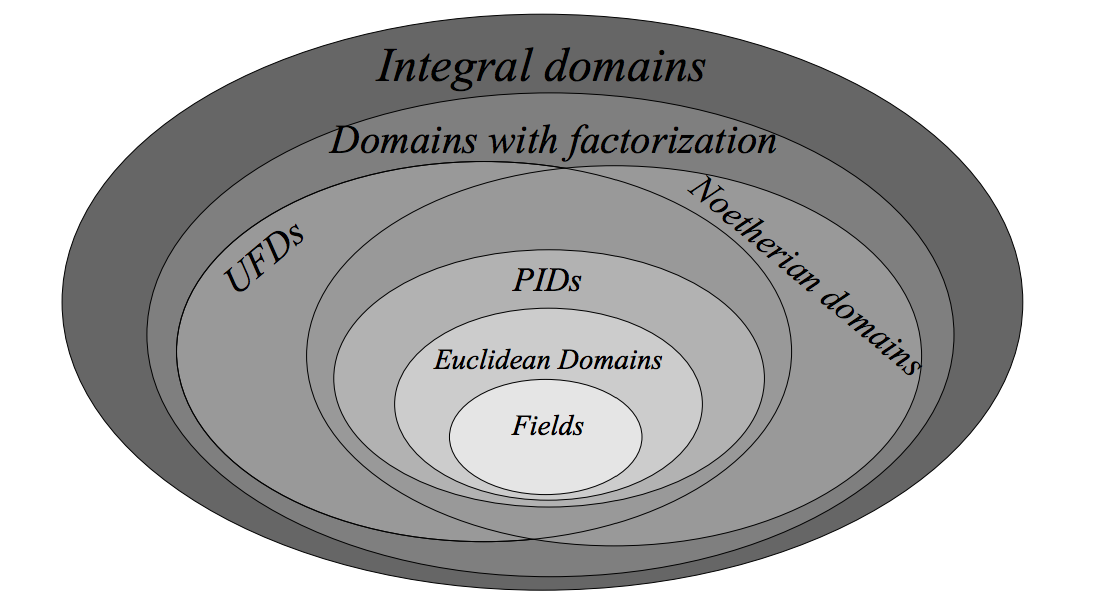
\includegraphics[width=\textwidth]{rings-aluffi.png}

 \section*{Definitions}
   \subsection*{Integral domain}
     The product of any nonzero elements is nonzero.
   \subsection*{Domain with factorization}
     Every nonzero non-unit element can be written as a finite product of irreducible elements.
   \subsection*{UFD}
     Every nonzero element can be written as a product of prime elements and a unit. Equivalently,
     every nonzero element can be written as an unique product (up to permutations and associates) of
     irreducible elements.
   \subsection*{Noetherian ring}
     Verifies the ascending chain condition on ideals. Any chain:
      \[ I_1 \subset I_2 \subset I_3 \subset \dots \subset I_n \subset \dots \]
     stabilizes after a finite number of steps.
   \subsection*{PID}
     Every ideal is principal (can be generated by a single element).
   \subsection*{Euclidean domain}
     Ring endowed with an euclidean function, a function $\Phi: R \rightarrow \mathbb{N}$ satisfiying:
     \[ \forall a,b \in R\setminus\{0\}: \exists q,r \in R: \quad a = bq + r \mbox{, and } \Phi(r) < \Phi(b) \]
   \subsection*{Field}
     Every element has an inverse.
    
 \section*{Examples}
   \subsection*{Integral domain}
     \[ \mathbb{K}\left[x,x^{\frac{1}{2}},x^{\frac{1}{4}}, \dots\right] \]
   \subsection*{Domain with factorization:}
     \[ \mathbb{Z}\left[\sqrt{-5}\right] \]
   \subsection*{UFD:}
     \[ \mathbb{K}\left[x_1,x_2,x_3\dots\right] \]
   \subsection*{Noetherian ring:}
     \[ \mathbb{Z}[x] \]
   \subsection*{PID:}
     \[ \mathbb{Z}\left[\scriptstyle{\frac{1+\sqrt{19}}{2}}\right] \]
   \subsection*{Euclidean domain:}
     \[ \mathbb{Z} \]
   \subsection*{Field:}
     \[ \mathbb{Q} \]
\end{document}